\documentclass[a4paper]{article}
\usepackage[utf8]{inputenc}
\usepackage[T1]{fontenc}
\usepackage[magyar]{babel}
\usepackage{lmodern}

%underbracket
\usepackage{amsmath}
%\coloneqq
\usepackage{mathtools}
%multicol
\usepackage{multicol}
%margin
\usepackage[a4paper, total={7in, 10in}]{geometry}
%links
\usepackage{hyperref}
%captions
\usepackage[font=small,labelfont=bf]{caption}
\captionsetup{labelformat=empty}
%golang
\usepackage{listings}
\usepackage{listings-golang} % import this package after listings
\usepackage{color}
\definecolor{brown}{RGB}{178,141,103}
\definecolor{green-dark}{RGB}{94,153,85}
\lstset{
    language=Go,
	basicstyle=\ttfamily\footnotesize,
    numberstyle=\footnotesize,
    numbers=left,
    frame=single,
    tabsize=2,
    breaklines=true,
    breakatwhitespace=true,
    framextopmargin=2pt,
    framexbottommargin=2pt,
    inputencoding=utf8,
	extendedchars=true,
	showstringspaces=false,
	literate=
		{µ}{{$\mu$}}1,
	keywordstyle=\color{blue}\ttfamily,
	stringstyle=\color{brown}\ttfamily,
	commentstyle=\color{green-dark}\ttfamily,
}

\usepackage{subfigure}

\newcommand{\dd}[1]{\mathrm{d}#1}
\newcommand{\sgn}[0]{\mathrm{sgn}}
\newcommand{\undbr}[1]{\underbrace{#1 \vphantom{\left(\frac{a^{0.3}}{b}\right)}}}

\title{Töltés mozgása a rá merőleges mágneses térben, súrlódással}
\author{Vörös Asztrik}
\date{}

\begin{document}
\maketitle

\begin{abstract}
	Egy töltött részecske mozgását vizsgáltam a sebességére merőleges mágneses mezőben, ahol sebességtől lineárisan függő súrlódási erő hat rá, de nehézségi erő nem. A pályát egy adott, a mágneses mezőben szereplő kezdő pozíciótól kezdve határoztam meg egészen addig, amíg abból ki nem lép vagy egy szint alá nem lassul a sebessége. A problémát egyenletekkel válaszoltam meg, illetve a kilépést program segítségével állapítottam meg. Végül összevetettem a szimulált eredménnyel a precíz képletet.
\end{abstract}

\begin{multicols}{2}

\section{Súrlódás nélkül}
	\begin{center}
		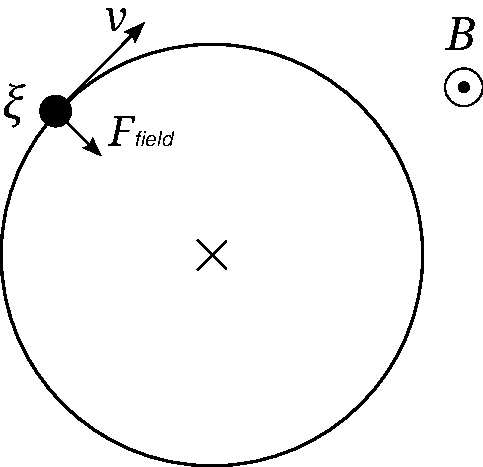
\includegraphics[height=10em]{graphics/base.pdf}
	\end{center}
	Mivel a mágneses mező vektora ($\vec{B}$) merőleges a töltött részecske ($\xi \coloneqq (m,q,\vec{v_0})$) sebességre ($\vec{v}$), így a mező ereje ($\vec{F_{\mathrm{field}}}$) síkban nézve merőleges lesz a sebességre. Ez a súrlódástól eltekintve körmozgást fog eredményezni, hiszen infinitezimálisan vizsgálva az erő csak a vektor irányát képes változtatni, a nagyságát nem, valamint a vektor irányának változásával a rá ható erő is vele együtt azonos irányba változik.

\section{Súrlódást bevezetve}
	\begin{center}
		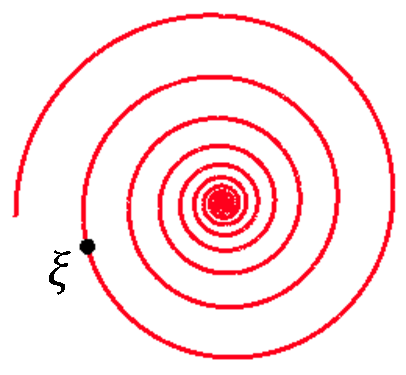
\includegraphics[height=10em]{graphics/spiral.pdf}
	\end{center}
	Ezen problémában egy a sebességtől lineárisan függő súrlódást ($F_{\mathrm{fric}}$) vezetünk be, így megjelenik a körmozgási probláma során ismert tangenciális erő, amely már hatással van a $\vec{v}$ nagyságára. Ebből egyrészt látszódik, hogy $\vec{v}$ függ az időtől ($t$), illetve mivel $F_{\mathrm{fric}}$ függ a sebességtől, így $F_{\mathrm{fric}}$ is függeni fog az időtől. Vezessük be a következő egyenletet a súrlódási erőre: $F_{\mathrm{fric}}(t) \coloneqq - \gamma v(t)$, ahol $\gamma$ egy pozitív együttható. \\
	Mivel $F_{\mathrm{field}}$ a körmozgásért felelős, így
	\begin{align*}
		F_{\mathrm{field}}(t) &= m \frac{v(t)^2}{r} \\
		qv(t)B\sin(90\deg) &= m \frac{v(t)^2}{r} \\
		r &= \frac{m}{qB} v(t) \\
		r(t) &\coloneqq \frac{m}{qB} v(t)
	\end{align*}
	Átrendezéssel látható, hogy a sugár is egy időtől függő tényező. Mivel a körmozgás feltételei a mozgás során teljesülnek, valamint a sugár folyamatosan csökken a sebesség csökkenése miatt, ezért egy spirálszerű mozgást kapunk.
	Hogy igazoljam feltevésemet, numerikus analízis segítségével közelítőleg ellenőrztem érvelésem 64 bites lebegő pontos számábrázolással, így az fenti képet kaptam, amely megerősítést tesz az eddigiekben. 

\section{Sebesség meghatározása}
	A súrlódás egyenletében észrevehetjük az alábbi elsőfokú szeparábilis lineáris differenciálegyenletet.
	\begin{align*}
		F_{s} &= - \gamma v(t) \\
		m \dot{v} &= - \gamma v(t) \\
		\dot{v} &= \undbr{- \frac{\gamma}{m}}_{f(t)} \undbr{v(t)}_{g(v(t))}
	\end{align*}
	Ennek egyensúlyi helyzetét ($g(v) \equiv 0$) a képletek végén kezeljük. Ezért tegyük fel, hogy $g(v) \neq 0$ és osszunk le vele.
	\vfill\pagebreak
	\begin{align*}
		\int \frac{v'(t)}{g(v(t))} \dd{t} &= \int f(t) \dd{t} \\
		\int \frac{v'(t)}{v(t)} \dd{t} &= \int - \frac{\gamma}{m} \dd{t} \\
		\ln |v(t)| &= - \frac{\gamma}{m} t + c \\
		|v(t)| &= \exp\left(- \frac{\gamma}{m} t + c \right) \\
			&= \exp\left(- \frac{\gamma}{m} t \right) \cdot \exp(c) \\
			&= \exp\left(- \frac{\gamma}{m} t \right) \cdot c \\
		v(t) &= \exp\left(- \frac{\gamma}{m} t \right) \cdot c
	\end{align*}
	Láthatjuk, hogy ha $c=0$, akkor az egyensúlyi helyzetet kaptuk vissza, ezért ez az általános képletünk. Most oldjuk, meg a Cauchy problémát, miszerint $v(0) = v_0$.
	\begin{align*}
		v(0) &= v_0 \\
		\exp(- \frac{\gamma}{m} \cdot 0 ) \cdot c &= v_0 \\
		c &= v_0
	\end{align*}

	\begin{center}
		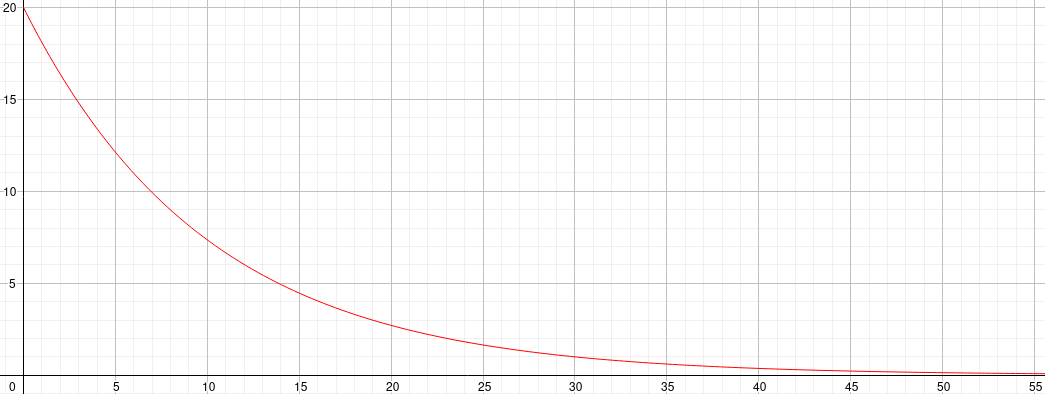
\includegraphics[width=\linewidth]{graphics/velocity.png}
	\end{center}

\section{Paraméteres görbe}
	\begin{center}
		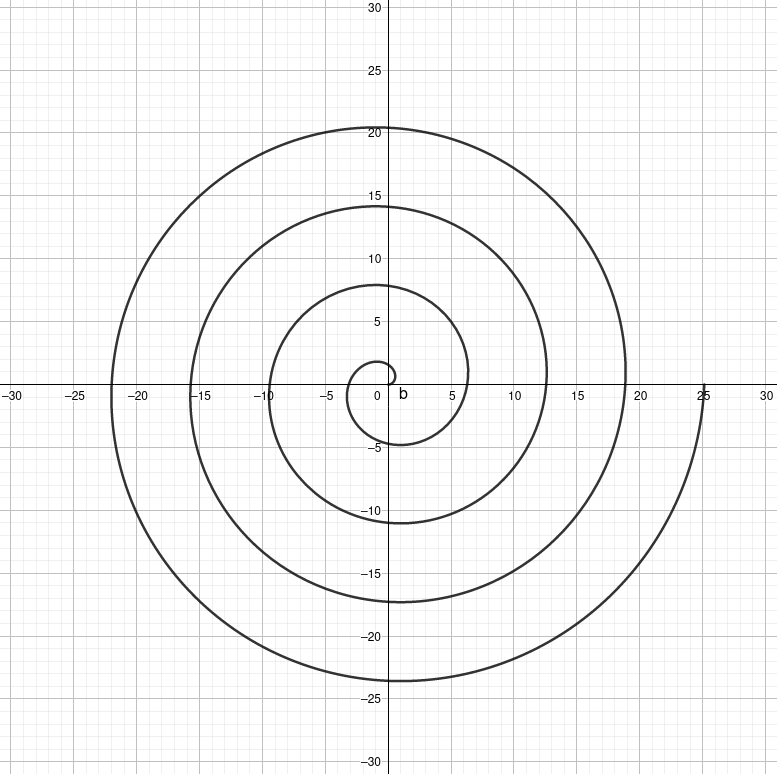
\includegraphics[height=10em]{graphics/parametric base.png}
	\end{center}
	Egy általam ismert paraméteres görbe az $(\alpha\cos(\alpha), \alpha\sin(\alpha))$, ahol megszabhatjuk $\alpha$-nak az értelmezési tartományát. Láthatjuk, hogy ebben az alakban könnyedén le tudjuk írni a pályát. \\
	A feladatunkhoz általánosítanunk kell a képletet és az idő szerint kifejeznünk a szöget, hiszen eddigi képleteinknek ez a paramétere. Feladatunkhoz a következő általánosítás megfelelő.
	\begin{align*}
		\begin{pmatrix}
			O_{x} + r(t) \cdot cos(\alpha_{0} \pm \int_{0}^{t} \omega(t) \dd{t})) \\
			O_{y} + r(t) \cdot sin(\alpha_{0} \pm \int_{0}^{t} \omega(t) \dd{t}))
		\end{pmatrix}
	\end{align*}
	
	\subsection{Középpont}
		Ezzel tudjuk az alakzatot az origóból eltolni. Ehhez vesszük a kezdeti pozíciót ($(x_0, y_0)$) és az abból kiinduló mező erejét, amit a kezdeti sugár méretére skálázunk át.
		\begin{align*}
			O &\coloneqq (x_{0}, y_{0}) + \vec{F_{\mathrm{field}}(0)} \frac{r(0)}{F_{\mathrm{field}}(0)}
		\end{align*}

	\subsection{$\alpha_{0}$}
		A paraméteres görbék a polárkoordinátás felírás szerint működnek ($(r\cos(\alpha), r\sin(\alpha))$), ezért meg kell határoznunk az alakzat középontjából számított kezdeti szöget ($\alpha_{0}$), hogy a paraméteres görbe $t=0$ esetén a kezdeti Descartes koordinátát adja meg. \\
		Jelölje $(\dd{x}, \dd{y})$ az alakzat középpontjából vett kezdeti pozíció koordinátáit. 
		\begin{align*}
			\dd{x} &\coloneqq x_0-O_{x} \\
			\dd{y} &\coloneqq y_0-O_{y}
		\end{align*}
		A polár koordinátáról a következő képpen térünk át:
		\begin{align*}
			r \cos(\alpha_{0}) = \dd{x} \\
			r \sin(\alpha_{0}) = \dd{y}
		\end{align*}
		Inverz függvény alkalmazásával nem pontosan kapjuk meg a szöget, hiszen a megfelelő tengelyre tükrözve is ugyanazt az eredményt adják a használt trigonometrikus függvények, azaz azok inverzei nem fedik le a teljes eredeti értelmezési tartományt. \\
		A kettőt együtt felhasználva azonban pontosan megadhatjuk a szöget ($[0,2\pi)$-n). A \textit{cos} az $x$ tengelyre tükrözött értékeket nem tudja megkülönböztetni, azonban ezt az \textit{arcsin} előjelével meg tudjuk állapítani, hiszen az negatív szöget ad eredményül, ha a paramétere negatív $\Leftrightarrow$ $y < 0$ $\Leftrightarrow$ $x$ tengely alatt van.
		\begin{align*}
			\alpha_{0_{\cos}} &\coloneqq \arccos \left( \frac{\dd{x}}{r} \right) \\
			\alpha_{0_{\sin}} &\coloneqq \arcsin \left( \frac{\dd{y}}{r} \right) \\
			\alpha &= \left\{
				\begin{array}{rl}
					\alpha_{0_{\cos}} & \textrm{ha } \alpha_{0_{\sin}} = 0 \\
					\sgn(\alpha_{0_{\sin}}) \cdot \alpha_{0_{\cos}} & \textrm{egyébként}
				\end{array}
			\right.
		\end{align*}

	\subsection{Forgási irány ($\pm$)}
		\newcommand{\vecFrom}[0]{v_{\mathrm{from}}}
		\newcommand{\vecTo}[0]{v_{\mathrm{to}}}
		\begin{center}
			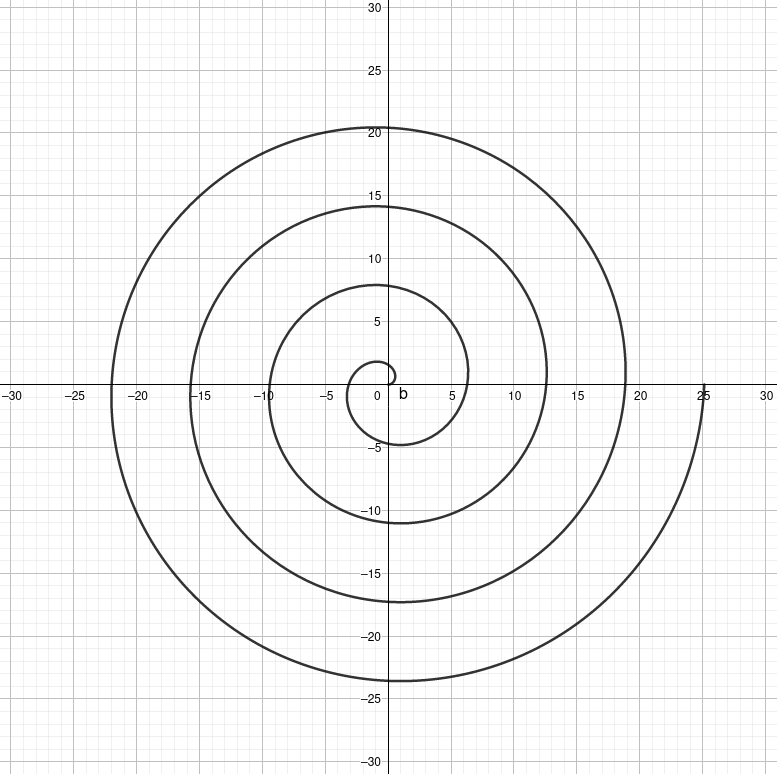
\includegraphics[height=10em]{graphics/parametric base.png}
			\quad
			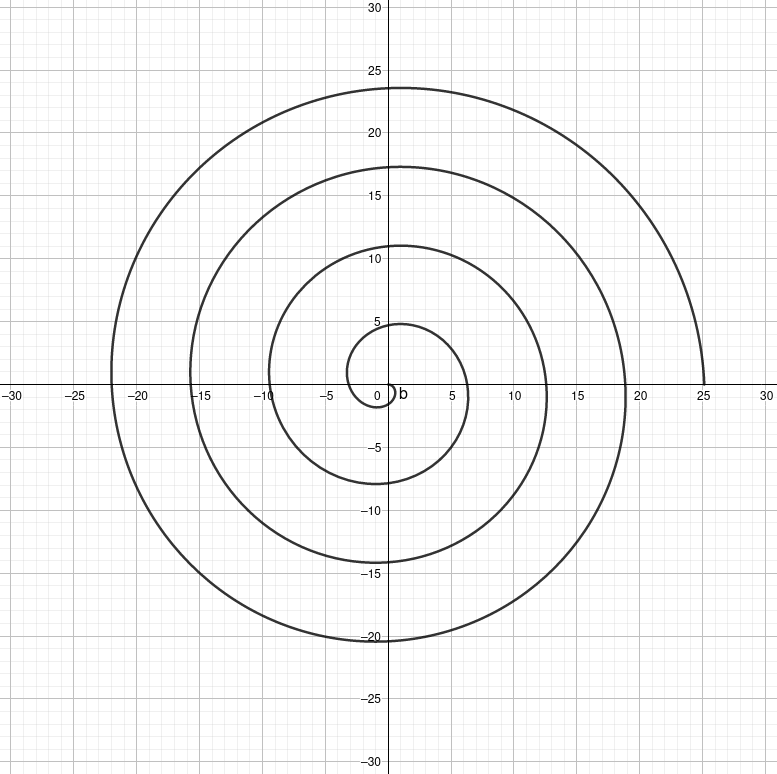
\includegraphics[height=10em]{graphics/parametric direction.png}
		\end{center}
		Azt kell megállapítanunk, hogy $\vec{v(0)}$ pozitív forgásba indítja el a részecskét vagy negatívba, hiszen ez a folyamat során nem változik. Ezzel ekvivalens probléma ha megállapítjuk, hogy $\vec{r(0)}$-hoz képest $\vec{v(0)}$ balra vagy jobbra helyezkedik el. \\
		Ehhez egy, a programozási versenyeken használatos geometriai algoritmust használtam. \\
		\begin{align*}
			\vec{\vecFrom} &\coloneqq \vec{r(0)} \\
			\vec{\vecTo} &\coloneqq \vec{v(0)} \\
			T &\coloneqq {\vecFrom}_y \cdot {\vecTo}_x - {\vecFrom}_x \cdot {\vecTo}_y \\
			\mathrm{direction} &= \left\{
				\begin{array}{rl}
					- & T > 0 \\
					+ & T < 0 \\
					0 & T = 0 \\
				\end{array}
			\right.
		\end{align*}
		A területből az irányra való következtetés bizonyítása az egyik előjelre (ekvivalens átalakítások):\\
		\begin{center}
			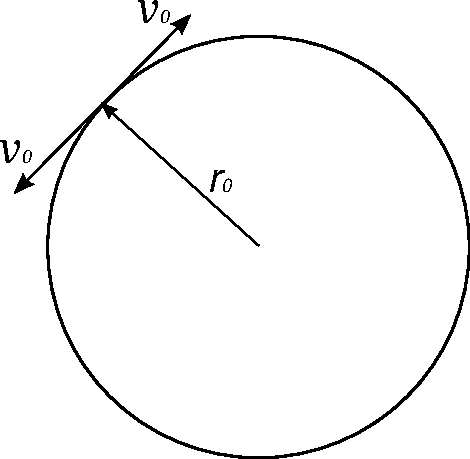
\includegraphics[height=10em]{graphics/direction.pdf}
			\quad
			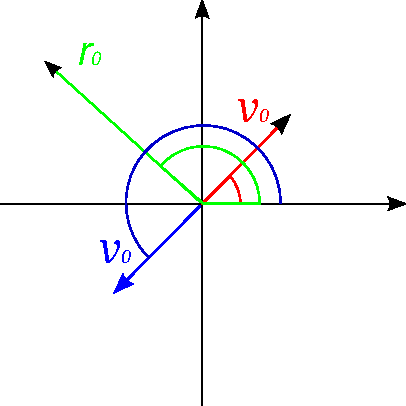
\includegraphics[height=10em]{graphics/direction origo.pdf}
		\end{center}
		\begin{align*}
			\alpha_{\mathrm{from}} &> \alpha_{\mathrm{to}} \\
			\tan{\alpha_{\mathrm{from}}} &> \tan{\alpha_{\mathrm{to}}} \\
			\frac{{\vecFrom}_y}{{\vecFrom}_x} &> \frac{{\vecTo}_y}{{\vecTo}_x} \\
			{\vecFrom}_y {\vecTo}_x &> {\vecTo}_y {\vecFrom}_x \\
			{\vecFrom}_y {\vecTo}_x - {\vecTo}_y {\vecFrom}_x &> 0
		\end{align*}

	\subsection{$\omega(t)$}
		Végül az adott pillanatra vonatkozó szögsebességet kell már csak megállapítani a következő összefüggéssel.
		\begin{align*}
			\omega(t) &= \frac{v(t)}{r(t)} \\
				&= \frac{q B}{m}
		\end{align*}
		Láthatjuk, hogy $\omega$ nem függ az időtől, így az integrálást könnyen el tudjuk végezni:
		\begin{align*}
			\int_{0}^{t} \omega(t) \dd{t} = \omega t
		\end{align*}

\section{Pálya vége}
	Mivel \textit{exp} sose éri el a $0$-át, ezért érdemes egy alsó korlátot bevezeti $v$-re ($v_{\mathrm{bound}}$).
	\begin{align*}
		v(t) > v_{\mathrm{bound}} \\
		\exp(-\frac{\gamma}{m}t) \cdot v_0 > v_{\mathrm{bound}} \\
		\exp(-\frac{\gamma}{m}t) > \frac{v_{\mathrm{bound}}}{v_0} \\
		-\frac{\gamma}{m}t > \ln\left( \frac{v_{\mathrm{bound}}}{v_0} \right) \\
		t < -\frac{m}{\gamma} \ln\left( \frac{v_{\mathrm{bound}}}{v_0} \right)
	\end{align*}
	Másik pályát megszakító tényező az az, hogyha a részecske kimegy a mágneses mezőből. Ezt nem precízen, program segítségével állapítottam meg, így ennek pontosság függ az időfelbontásától is.

\end{multicols}

\section{Program}
	A fentebb említett program \textit{config.json} fájl alapján vezérelhető. Lefutása során képként lementi piros színnel a szimulált pályát és zöld színnel a formulával kapott pályát. Érdemes megfigyelni alacsony időfelbontás mellett is az eltérést.
	\begin{figure}[h]
		\centering
		\begin{minipage}{0.25\textwidth}
			\centering
			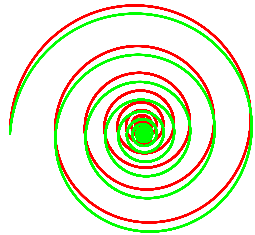
\includegraphics[height=7em]{graphics/result/result-1ms.png}
			\captionof{figure}{1ms}
		\end{minipage}%
		\begin{minipage}{0.25\textwidth}
			\centering
			\includegraphics[height=7em]{graphics/result/result-500µs.png}
			\captionof{figure}{500µs}
		\end{minipage}%
		\begin{minipage}{0.25\textwidth}
			\centering
			\includegraphics[height=7em]{graphics/result/result-250µs.png}
			\captionof{figure}{250µs}
		\end{minipage}%
		\begin{minipage}{0.25\textwidth}
			\centering
			\includegraphics[height=7em]{graphics/result/result-100µs.png}
			\captionof{figure}{100µs}
		\end{minipage}
	\end{figure}
	\begin{figure}[h]
		\centering
		\begin{minipage}{0.25\textwidth}
			\centering
			\includegraphics[height=7em]{graphics/result/result-50µs.png}
			\captionof{figure}{50µs}
		\end{minipage}%
		\begin{minipage}{0.25\textwidth}
			\centering
			\includegraphics[height=7em]{graphics/result/result-25µs.png}
			\captionof{figure}{25µs}
		\end{minipage}%
		\begin{minipage}{0.25\textwidth}
			\centering
			\includegraphics[height=7em]{graphics/result/result-10µs.png}
			\captionof{figure}{10µs}
		\end{minipage}
	\end{figure}\\
	Szintén kapunk egy formulát, melyet \href{https://www.geogebra.org/m/fsurybdc}{ezen geogebra sémát} felhasználva még le is játszhatjuk a mozgást. \\
	\fbox{\parbox{\textwidth}{
		Curve((143.333333 + 1.000000/(5.000000*0.300000) * e\^{}(-0.100000/1.000000 * t) * 200.000000 * cos(3.141593 - 1.500000 * t),101.000000 + 1.000000/(5.000000*0.300000) * e\^{}(-0.100000/1.000000 * t) * 200.000000 * sin(3.141593 - 1.500000 * t)),t,0,122.061000)
	}} \\
	\\
	Az elkövetkezőekben a forráskódot láthatjuk, ahol az elvégzett számítások már le vannak dokumentálva az előbbiekben, így kevésbé szerepelnek kommentek ott, ahol egyértelmű az elvégzett számítás oka.
	\lstinputlisting[caption=config.json]{../config.json}
	\lstinputlisting[caption=main.go]{../main.go}
	\lstinputlisting[caption=vector/vector.go]{../vector/vector.go}
	\lstinputlisting[caption=physics/config.go]{../physics/config.go}
	\lstinputlisting[caption=physics/friction.go]{../physics/friction.go}
	\lstinputlisting[caption=physics/magnetic-field.go]{../physics/magnetic-field.go}
	\lstinputlisting[caption=physics/particle.go]{../physics/particle.go}
	\lstinputlisting[caption=draw/draw.go]{../draw/draw.go}

\section{Források}
	\begin{itemize}
		\item Koordinátarendszeres képek: \href{https://www.geogebra.org/}{Geogebra}
	\end{itemize}
 
\end{document}